\documentclass[aspectratio=169,10pt]{beamer}
\usepackage[utf8]{inputenc}
\usepackage[T1]{fontenc}
\usepackage{amsmath,amssymb,amsthm}
\usepackage{graphicx}
\usepackage{listings}
\usepackage{xcolor}
\usepackage{tikz}
\usetikzlibrary{arrows.meta,positioning}
\usepackage{algorithm}
\usepackage{algorithmic}
\usepackage{hyperref}
\usepackage{mimic}

% Theme settings
\usetheme{Madrid}
\usecolortheme{seahorse}
\setbeamertemplate{navigation symbols}{}
\setbeamertemplate{footline}[frame number]

% Code listing configuration
\lstset{
    language=Python,
    basicstyle=\ttfamily\scriptsize,
    keywordstyle=\color{blue}\bfseries,
    stringstyle=\color{red},
    commentstyle=\color{green!60!black},
    showstringspaces=false,
    breaklines=true,
    breakatwhitespace=true,
    frame=single,
    numbers=left,
    numberstyle=\tiny\color{gray},
    xleftmargin=1em,
    framexleftmargin=1em
}

% Title page information
\title{Reinforcement Learning}
\subtitle{Lecture 7: DQN Project (CartPole Case Study)}
\author{Taehoon Kim}
\institute{Sogang University MIMIC Lab \\ \url{https://mimic-lab.com}}
\date{Fall Semester 2025}

\begin{document}

% Slide 1: Title
\frame{\titlepage}

% Slide 2: Today's Agenda
\begin{frame}{Today's Agenda}
\begin{itemize}
    \item Review DQN architecture and revisit prior experiments
    \item Diagnose overfitting and instability in value-based deep RL
    \item Walk through implementation building blocks (buffer, network, training loop)
    \item Compare advanced DQN variants and interpret real experiments
    \item Practice debugging workflows and consolidate project takeaways
\end{itemize}
\vspace{0.5em}
\textit{We will close with a live code walkthrough from \texttt{exp09\_complete\_dqn\_project.py} to demonstrate the debugging workflow end-to-end.}
\end{frame}

\section{Hands-on Experiments}

\begin{frame}{Section Overview: Hands-on Experiments}
\begin{block}{Structure}
\begin{itemize}
    \item Nine runnable scripts (\texttt{exp01}--\texttt{exp09}) build the DQN project incrementally
    \item Each slide pair details objectives, tasks, and expected outputs
    \item Artifacts land in \texttt{experiments/figures/}, \texttt{runs/}, or run-specific checkpoint folders
\end{itemize}
\end{block}
\begin{alertblock}{Execution Tips}
\begin{itemize}
    \item Activate the virtual environment and export deterministic env vars before sweeps
    \item Use \texttt{python lecture07/experiments/exp09\_integrated\_test.py} for end-to-end validation
\end{itemize}
\end{alertblock}
\end{frame}

\begin{frame}{Experiment Scripts}
\begin{itemize}
    \item \texttt{exp01\_environment\_setup.py}: Verify env, device, seeding \textit{(instrumentation + reproducibility)}
    \item \texttt{exp02\_q\_learning\_basics.py}: Bellman update and Q-net demo \textit{(tabular vs. neural view)}
    \item \texttt{exp03\_replay\_buffer.py}: Circular buffer and sampling analysis \textit{(data decorrelation)}
    \item \texttt{exp04\_dqn\_network.py}: Architectures, target updates, inits \textit{(model capacity sweeps)}
    \item \texttt{exp05\_training\_loop.py}: End-to-end DQN training loop \textit{(buffer $\rightarrow$ optimizer)}
    \item \texttt{exp06\_hyperparameter\_tuning.py}: LR/batch/target sweeps \textit{(search automation)}
    \item \texttt{exp07\_advanced\_dqn.py}: Double/Dueling comparisons \textit{(variant ablations)}
    \item \texttt{exp08\_debugging\_visualization.py}: Gradients and Q diagnostics \textit{(failure triage)}
    \item \texttt{exp09\_complete\_dqn\_project.py}: Integrated DQN project \textit{(production checklist)}
\end{itemize}
\end{frame}

\begin{frame}{Expected Outputs}
\begin{itemize}
    \item Figures: \texttt{../experiments/figures/}
    \begin{itemize}
        \item \texttt{dqn\_training\_results.png} (from \texttt{exp05})
        \item \texttt{advanced\_dqn\_comparison.png} (from \texttt{exp07})
        \item \texttt{q\_value\_analysis.png}, \texttt{training\_diagnostics.png} (from \texttt{exp08})
    \end{itemize}
    \item Logs: \texttt{runs/} (from \texttt{exp09})
    \item Checkpoints: under each run directory (from \texttt{exp09})
\end{itemize}
\end{frame}

\begin{frame}{Learning Objectives}
\begin{block}{By the end of this lecture you will}
\begin{itemize}
    \item Implement and validate a DQN pipeline end-to-end (from buffer to evaluation)
    \item Understand and prevent overfitting in value-based RL
    \item Master hyperparameter tuning for DQN
    \item Implement advanced DQN variants (Double, Dueling)
    \item Create reproducible RL experiments
    \item Debug common DQN issues effectively
\end{itemize}
\end{block}

\begin{alertblock}{Prerequisites}
\begin{itemize}
    \item Understanding of Q-learning (Lecture 5)
    \item Basic DQN concepts (Lecture 6)
    \item PyTorch proficiency
\end{itemize}
\end{alertblock}
\end{frame}

\section{DQN Review and Project Setup}

\begin{frame}{Section Overview: DQN Review \& Setup}
\begin{block}{Goals}
\begin{itemize}
    \item Revisit the DQN building blocks before deep dives
    \item Ground the CartPole case study in environment specs and reproducibility
    \item Align code folders, helper utilities, and artifact layout
\end{itemize}
\end{block}
\begin{alertblock}{Keep in Mind}
\begin{itemize}
    \item Slides cite code from \texttt{exp04}--\texttt{exp06}
    \item Deterministic seeds (\texttt{setup\_seed}) and device helpers carry into every lab
\end{itemize}
\end{alertblock}
\end{frame}

% Slide 5: DQN Architecture Recap
\begin{frame}{DQN Architecture Recap}
\begin{columns}
\column{0.5\textwidth}
\textbf{Key Components:}
\begin{itemize}
    \item Neural network Q-function
    \item Experience replay buffer
    \item Target network
    \item $\epsilon$-greedy exploration
\end{itemize}

\column{0.5\textwidth}
\textbf{Update Rule:}
\begin{align}
y &= r + \gamma \max_{a'} Q_{\theta^-}(s', a') \\
\mathcal{L}(\theta) &= \mathbb{E}_{(s,a,r,s',d) \sim \mathcal{D}} \left[ H_\kappa(y - Q_\theta(s,a)) \right]
\end{align}
where $H_\kappa$ is Huber loss

{\footnotesize $H_\kappa$ denotes the piecewise smooth $L_1$ loss, reducing sensitivity to outliers in TD errors.}
\end{columns}
\end{frame}

% Slide 6: CartPole Environment
\begin{frame}{CartPole-v1 Environment}
\begin{columns}
\column{0.5\textwidth}
\textbf{Observation Space:}
\begin{itemize}
    \item Cart position: $x \in [-4.8, 4.8]$
    \item Cart velocity: $\dot{x} \in [-\infty, \infty]$
    \item Pole angle: $\theta \in [-0.418, 0.418]$ rad
    \item Pole angular velocity: $\dot{\theta} \in [-\infty, \infty]$
\end{itemize}

\column{0.5\textwidth}
\textbf{Action Space:}
\begin{itemize}
    \item 0: Push cart to the left
    \item 1: Push cart to the right
\end{itemize}

\textbf{Reward:}
\begin{itemize}
    \item +1 for each step the pole remains upright
    \item Episode ends if pole falls or cart leaves bounds
\end{itemize}
\end{columns}
\end{frame}

% Slide 7: Project Structure
\begin{frame}[fragile]{Project Structure}
\begin{lstlisting}
DQN_Project/
|-- experiments/
|   |-- exp01_environment_setup.py
|   |-- exp02_q_learning_basics.py
|   |-- exp03_replay_buffer.py
|   |-- exp04_dqn_network.py
|   |-- exp05_training_loop.py
|   |-- exp06_hyperparameter_tuning.py
|   |-- exp07_advanced_dqn.py
|   |-- exp08_debugging_visualization.py
|   |-- exp09_complete_dqn_project.py
|-- runs/              # TensorBoard logs
|-- checkpoints/       # Model checkpoints
\end{lstlisting}
\end{frame}

% Slide 8: Reproducibility Setup
\begin{frame}[fragile]{Reproducibility Setup}
\begin{lstlisting}
def setup_seed(seed=42):
    random.seed(seed)
    np.random.seed(seed)
    torch.manual_seed(seed)
    if torch.cuda.is_available():
        torch.cuda.manual_seed_all(seed)

device = torch.device(
    'cuda' if torch.cuda.is_available() 
    else 'mps' if hasattr(torch.backends, 'mps') and torch.backends.mps.is_available()
    else 'cpu'
)
\end{lstlisting}
\textbf{Key: Consistent seeding across all libraries}
\end{frame}

% Slide 9: Reproducibility Checklist
\begin{frame}{Reproducibility Checklist}
\begin{itemize}
    \item[$\square$] Fixed seeds for Python, NumPy, PyTorch
    \item[$\square$] Environment reset with deterministic seed (e.g., \texttt{state, info = env.reset(seed=42)})
    \item[$\square$] Library versions documented
    \item[$\square$] Hardware information logged
    \item[$\square$] Configuration saved with unique hash
    \item[$\square$] Checkpoints include RNG states
    \item[$\square$] TensorBoard logging enabled
    \item[$\square$] Evaluation uses fixed seeds
\end{itemize}
\textbf{Goal: Anyone can reproduce your results exactly}
\end{frame}

\section{Overfitting and Instability}

\begin{frame}{Section Overview: Overfitting \& Instability}
\begin{block}{Key Questions}
\begin{itemize}
    \item How do we recognize when value-based agents memorize replay data?
    \item Which metrics from \texttt{exp05}--\texttt{exp07} flag brittle policies?
    \item What mitigation knobs (data, network, regularizers) should we reach for first?
\end{itemize}
\end{block}
\begin{alertblock}{Artifacts Referenced}
\begin{itemize}
    \item Training curves + diagnostics: \texttt{exp05\_training\_loop.py}
    \item Variant ablations: \texttt{exp07\_advanced\_dqn.py}
\end{itemize}
\end{alertblock}
\end{frame}

% Slide 11: Overfitting in RL
\begin{frame}{Overfitting in Value-Based RL}
\textbf{Three Common Symptoms:}
\begin{enumerate}
    \item Loss oscillates despite sufficient data
    \item Greedy policy becomes brittle after improvement
    \item Performance varies strongly across seeds
\end{enumerate}

\vspace{1em}
\textbf{Causes:}
\begin{itemize}
    \item Agent exploits narrow replay window
    \item Memorizes recent transitions
    \item Fails to generalize to full on-policy distribution
    \item Replay buffer sampling bias limits coverage
    \item Non-stationary targets (policy + target net drift)
\end{itemize}
\end{frame}

% Slide 12: Remedies for Overfitting
\begin{frame}{Remedies for Overfitting}
\begin{columns}
\column{0.5\textwidth}
\textbf{Data Diversity:}
\begin{itemize}
    \item Large replay buffer
    \item Diverse exploration
    \item Stratified sampling
    \item Data augmentation (for image observations)
\end{itemize}

\textbf{Network Stability:}
\begin{itemize}
    \item Target network
    \item Soft updates
    \item Gradient clipping
\end{itemize}

\column{0.5\textwidth}
\textbf{Regularization:}
\begin{itemize}
    \item Huber loss
    \item Reward scaling
    \item Early stopping
\end{itemize}

\textbf{Architecture:}
\begin{itemize}
    \item Appropriate capacity
    \item Dropout (use carefully; can harm temporal consistency)
    \item Batch normalization
\end{itemize}
\end{columns}
\end{frame}

% Slide 13: Target Network Mechanism
\begin{frame}{Target Network Mechanism}
\textbf{Problem: Moving target instability}
\begin{itemize}
    \item Q-learning target depends on network being updated
    \item Creates feedback loop and oscillations
\end{itemize}

\vspace{1em}
\textbf{Solution: Frozen target network}
\begin{align}
    y = r + \gamma\, \max_{a'} Q_{\theta^-}(s', a')
\end{align}

where $\theta^-$ is periodically updated:
\begin{itemize}
    \item Hard update: $\theta^- \leftarrow \theta$ every $C$ steps
    \item Soft update: $\theta^- \leftarrow \tau\theta + (1-\tau)\theta^-$
\end{itemize}
\end{frame}

% Slide 14: Experience Replay Benefits
\begin{frame}{Experience Replay Benefits}
\begin{columns}[T]
\column{0.52\textwidth}
\textbf{Decorrelation}
\begin{itemize}
    \item Breaks temporal correlations in data
    \item Enables i.i.d.\ sampling assumption
    \item Stabilizes gradient estimates
\end{itemize}

\textbf{Data Efficiency}
\begin{itemize}
    \item Reuses experiences multiple times
    \item Enables off-policy learning
    \item Smooths learning over rare events
\end{itemize}

\column{0.48\textwidth}
\centering
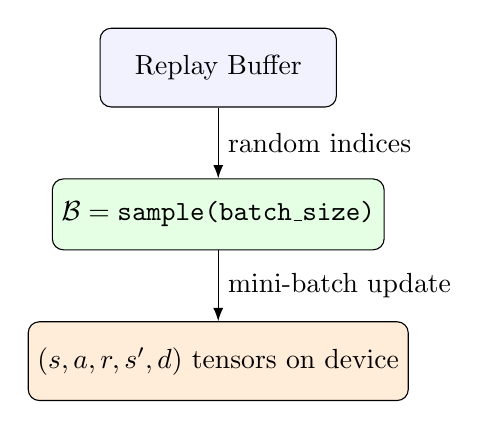
\begin{tikzpicture}[>=Latex,node distance=0.9cm]
\node[draw,rounded corners,minimum width=3cm,minimum height=1cm,fill=blue!5] (buffer) {Replay Buffer};
\node[draw,rounded corners,minimum width=2.8cm,minimum height=0.9cm,below=of buffer,fill=green!10] (batch) {$\mathcal{B}=\texttt{sample(batch\_size)}$};
\node[draw,rounded corners,minimum width=3.4cm,minimum height=1cm,below=of batch,fill=orange!15] (tensors) {$(s,a,r,s',d)$ tensors on device};
\draw[->] (buffer) -- node[right]{random indices} (batch);
\draw[->] (batch) -- node[right]{mini-batch update} (tensors);
\end{tikzpicture}

{\scriptsize See \texttt{ReplayBuffer.sample()} in \texttt{exp03\_replay\_buffer.py}.}
\end{columns}
\end{frame}

\section{Preprocessing and Hyperparameters}

\begin{frame}{Section Overview: Preprocessing \& Hyperparameters}
\begin{block}{What We Cover}
\begin{itemize}
    \item Minimal preprocessing choices for CartPole vs. image domains
    \item Sensitivity ranking for LR, batch size, target update, exploration
    \item How \texttt{exp05} and \texttt{exp06} log sweeps for reproducibility
\end{itemize}
\end{block}
\begin{alertblock}{Link to Experiments}
\begin{itemize}
    \item Hyperparameter sweeps: \texttt{exp06\_hyperparameter\_tuning.py}
    \item Training loop knobs: \texttt{exp05\_training\_loop.py}
\end{itemize}
\end{alertblock}
\end{frame}

% Slide 16: Preprocessing Pipeline
\begin{frame}[fragile]{Preprocessing Pipeline}
\textbf{Common Preprocessing Steps:}
\begin{enumerate}
    \item Frame skipping (action repeat)
    \item Frame stacking (temporal context)
    \item Reward scaling/clipping
    \item State normalization
\end{enumerate}

\vspace{1em}
\textbf{For CartPole:}
\begin{itemize}
    \item Minimal preprocessing needed (already low-dimensional)
    \item Optional: state normalization
    \item Optional: frame stacking for velocity estimation
\end{itemize}

\begin{exampleblock}{State normalization in \texttt{exp05\_training\_loop.py}}
\begin{lstlisting}
state = torch.from_numpy(state).float()
state = (state - obs_rms.mean) / (obs_rms.var.sqrt() + 1e-8)
\end{lstlisting}
\end{exampleblock}
\end{frame}

% Slide 17: Key Hyperparameters
\begin{frame}{Key Hyperparameters in DQN}
\begin{columns}[T]
\column{0.52\textwidth}
\textbf{Learning Dynamics}
\begin{itemize}
    \item Learning rate: $10^{-4}$ to $10^{-3}$
    \item Batch size: 32 to 256
    \item Gradient clipping: 10.0
\end{itemize}

\textbf{Exploration}
\begin{itemize}
    \item $\epsilon$ start: 1.0, end: 0.01–0.1
    \item Schedules: linear, exponential, or stepped
\end{itemize}

\textbf{Memory \& Updates}
\begin{itemize}
    \item Buffer size: 10K–100K
    \item Target update: 500–10K steps
    \item Discount $\gamma$: 0.99
\end{itemize}

\textbf{Network}
\begin{itemize}
    \item Hidden dimensions: 128–256
    \item Activation: ReLU; Optimizer: Adam
\end{itemize}

\column{0.48\textwidth}
\textbf{Exploration schedules (visualized)}
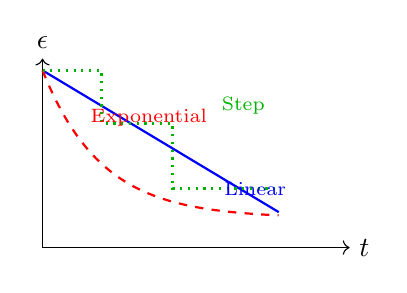
\begin{tikzpicture}[scale=0.75]
\draw[->] (0,0) -- (5.2,0) node[right] {$t$};
\draw[->] (0,0) -- (0,3.2) node[above] {$\epsilon$};
\draw[thick,blue] (0,3) -- (4,0.6);
\draw[thick,red,dashed,domain=0:4,samples=50] plot (\x,{0.5+2.5*exp(-\x)});
\draw[thick,green!70!black,dotted] (0,3) -- (1,3) -- (1,2.1) -- (2.2,2.1) -- (2.2,1) -- (4,1);
\node[blue] at (3.6,1.0) {\scriptsize Linear};
\node[red] at (1.8,2.2) {\scriptsize Exponential};
\node[green!70!black] at (3.4,2.4) {\scriptsize Step};
\end{tikzpicture}
\end{columns}
\end{frame}

% Slide 18: Hyperparameter Sensitivity
\begin{frame}{Hyperparameter Sensitivity Analysis}
\textbf{Most Critical (High Impact):}
\begin{itemize}
    \item Learning rate: Too high $\rightarrow$ instability
    \item Target update frequency: Balance stability vs staleness
    \item Exploration schedule: Coverage vs exploitation
\end{itemize}

\vspace{1em}
\textbf{Moderately Important:}
\begin{itemize}
    \item Batch size: Gradient variance
    \item Buffer size: Sample diversity
    \item Network capacity: Expressiveness (too large $\rightarrow$ slower convergence, overfitting risk)
\end{itemize}

\vspace{1em}
\textbf{Less Sensitive:}
\begin{itemize}
    \item Gradient clipping threshold
    \item Optimizer momentum
\end{itemize}
\end{frame}


\section{Implementation Details}

\begin{frame}{Section Overview: Implementation Details}
\begin{block}{Focus Areas}
\begin{itemize}
    \item Replay buffer memory layout and sampling logic
    \item Network definitions + loss computation snippets (\texttt{exp04}, \texttt{exp05})
    \item Training loop scaffolding (epsilon decay, device transfers, tensor shapes)
\end{itemize}
\end{block}
\begin{alertblock}{Remember}
\begin{itemize}
    \item Add \texttt{[fragile]} when slides show code listings
    \item Reference exact helper names to mirror the experiments
\end{itemize}
\end{alertblock}
\end{frame}

% Slide 21: Replay Buffer Implementation
\begin{frame}[fragile]{Efficient Replay Buffer}
\begin{lstlisting}
class ReplayBuffer:
    def __init__(self, state_dim, capacity, device):
        self.capacity = capacity
        self.pos = 0
        self.full = False
        # Pre-allocate arrays for efficiency
        self.states = np.zeros((capacity, state_dim), dtype=np.float32)
        self.actions = np.zeros(capacity, dtype=np.int64)
        self.rewards = np.zeros(capacity, dtype=np.float32)
        self.next_states = np.zeros((capacity, state_dim), dtype=np.float32)
        self.dones = np.zeros(capacity, dtype=np.bool8)
\end{lstlisting}
\textbf{Key: Pre-allocation for memory efficiency}
\end{frame}

% Slide 22: Circular Buffer Logic
\begin{frame}[fragile]{Circular Buffer Logic}
\begin{lstlisting}
def add(self, state, action, reward, next_state, done):
    self.states[self.pos] = state
    self.actions[self.pos] = action
    self.rewards[self.pos] = reward
    self.next_states[self.pos] = next_state
    self.dones[self.pos] = done
    
    self.pos = (self.pos + 1) % self.capacity
    self.full = self.full or self.pos == 0
    
def sample(self, batch_size):
    max_idx = self.capacity if self.full else self.pos
    idx = np.random.randint(0, max_idx, size=batch_size)
    # Returns (s, a, r, s', d) tensors on the target device
\end{lstlisting}
\end{frame}

% Slide 23: DQN Network Architecture
\begin{frame}[fragile]{DQN Network Architecture}
\begin{lstlisting}
class DQN(nn.Module):
    def __init__(self, state_dim, action_dim, hidden_dim=128):
        super().__init__()
        self.fc1 = nn.Linear(state_dim, hidden_dim)
        self.fc2 = nn.Linear(hidden_dim, hidden_dim)
        self.fc3 = nn.Linear(hidden_dim, action_dim)
    
    def forward(self, x):
        x = F.relu(self.fc1(x))  # [B, state_dim] -> [B, hidden]
        x = F.relu(self.fc2(x))  # [B, hidden] -> [B, hidden]
        x = self.fc3(x)          # [B, hidden] -> [B, action_dim]
        return x
\end{lstlisting}
\end{frame}

% Slide 24: Loss Computation
\begin{frame}[fragile]{DQN Loss Computation}
\begin{lstlisting}
def compute_loss(batch, policy_net, target_net, gamma):
    states, actions, rewards, next_states, dones = batch
    
    # Current Q values
    current_q = policy_net(states).gather(1, actions.unsqueeze(1)).squeeze(1)
    
    # Target Q values
    with torch.no_grad():
        next_q = target_net(next_states).max(1)[0]
        target_q = rewards + gamma * next_q * (1 - dones)
    
    # Huber loss for stability
    loss = F.smooth_l1_loss(current_q, target_q)
    return loss
\end{lstlisting}
\end{frame}

% Slide 25: Tensor Shape Tracking
\begin{frame}{Tensor Shape Tracking}
\textbf{Critical for debugging:}
\begin{itemize}
    \item States: [batch\_size, state\_dim]
    \item Actions: [batch\_size]
    \item Q-values: [batch\_size, action\_dim]
    \item Selected Q: [batch\_size]
    \item Targets: [batch\_size]
\end{itemize}

\vspace{1em}
\textbf{Common shape errors:}
\begin{itemize}
    \item Forgetting to squeeze/unsqueeze
    \item Mismatched batch dimensions
    \item Wrong gather dimension
\end{itemize}
\end{frame}

% Slide 26: Training Loop Structure
\begin{frame}[fragile]{Training Loop Structure}
\begin{lstlisting}
for episode in range(num_episodes):
    state, _ = env.reset()
    done = False
    
    while not done:
        # Select action (epsilon-greedy)
        action = select_action(state, epsilon)
        
        # Environment step (Gymnasium API)
        next_state, reward, terminated, truncated, _ = env.step(action)
        done = terminated or truncated  # Replaces legacy Gym "done" flag
        
        # Store and update
        memory.push(state, action, reward, next_state, done)
        loss = update_network()
        
        state = next_state
\end{lstlisting}
\end{frame}

% Slide 27: Epsilon Decay Strategies
\begin{frame}{Epsilon Decay Strategies}
\begin{columns}[T]
\column{0.55\textwidth}
\textbf{Linear}
\begin{align*}
\epsilon_t = \epsilon_{start} + t \cdot \frac{\epsilon_{end} - \epsilon_{start}}{T}
\end{align*}

\textbf{Exponential}
\begin{align*}
\epsilon_t = \epsilon_{end} + (\epsilon_{start} - \epsilon_{end}) e^{-t/\tau}
\end{align*}

\textbf{Step}
\begin{align*}
\epsilon_t = \epsilon_{start} \cdot \alpha^{\lfloor t/k \rfloor}
\end{align*}

\textbf{Guidance}
\begin{itemize}
    \item Linear: predictable annealing for small projects
    \item Exponential: fast drop, good for long horizons
    \item Step: coarse schedule for staged curricula
\end{itemize}

\column{0.45\textwidth}
\centering
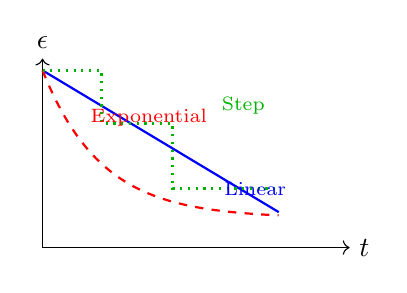
\begin{tikzpicture}[scale=0.75]
\draw[->] (0,0) -- (5.2,0) node[right] {$t$};
\draw[->] (0,0) -- (0,3.2) node[above] {$\epsilon$};
\draw[thick,blue] (0,3) -- (4,0.6);
\draw[thick,red,dashed,domain=0:4,samples=50] plot (\x,{0.5+2.5*exp(-\x)});
\draw[thick,green!70!black,dotted] (0,3) -- (1,3) -- (1,2.1) -- (2.2,2.1) -- (2.2,1) -- (4,1);
\node[blue] at (3.6,1.0) {\scriptsize Linear};
\node[red] at (1.8,2.2) {\scriptsize Exponential};
\node[green!70!black] at (3.4,2.4) {\scriptsize Step};
\end{tikzpicture}
\end{columns}
\end{frame}

\section{Diagnostics Snapshot}

\begin{frame}{Section Overview: Diagnostics Snapshot}
\begin{block}{Focus}
\begin{itemize}
    \item Surface quantitative evidence from \texttt{exp05}, \texttt{exp07}, and \texttt{exp08}
    \item Highlight observed metrics before diving into derivations
    \item Frame troubleshooting questions for the live walkthrough
\end{itemize}
\end{block}
\begin{alertblock}{Artifacts}
\begin{itemize}
    \item Figures stored under \texttt{../experiments/figures/}
    \item Console metrics captured alongside each experiment run
\end{itemize}
\end{alertblock}
\end{frame}





\section{Advanced DQN Variants}

\begin{frame}{Section Overview: Advanced Variants}
\begin{block}{Objectives}
\begin{itemize}
    \item Contrast vanilla DQN with Double and Dueling implementations
    \item Clarify when soft vs. hard target updates help stability
    \item Tie back to metrics plotted in \texttt{exp07\_advanced\_dqn.py}
\end{itemize}
\end{block}
\begin{alertblock}{Scripts Referenced}
\begin{itemize}
    \item \texttt{exp07\_advanced\_dqn.py} (variant sweeps)
    \item \texttt{exp04\_dqn\_network.py} (architecture definitions)
\end{itemize}
\end{alertblock}
\end{frame}

% Slide 29: Double DQN
\begin{frame}{Double DQN}
\textbf{Problem: Overestimation bias}
\begin{itemize}
    \item Standard DQN: $\max$ operator causes systematic overestimation
    \item Accumulates over iterations
\end{itemize}

\vspace{1em}
\textbf{Solution: Decouple selection and evaluation}
\begin{align}
a^\star &= \arg\max_a Q_\theta(s', a) \quad \text{(selection)} \\
y &= r + \gamma Q_{\theta^-}(s', a^\star) \quad \text{(evaluation)}
\end{align}

\textbf{Result: Reduced bias, more stable learning}
\end{frame}

% Slide 30: Double DQN Implementation
\begin{frame}[fragile]{Double DQN Implementation}
\begin{lstlisting}
# Standard DQN
with torch.no_grad():
    next_q = target_net(next_states).max(1)[0]
    target_q = rewards + gamma * next_q * (1 - dones)

# Double DQN
with torch.no_grad():
    # Use policy network to select actions
    next_actions = policy_net(next_states).argmax(1)
    # Use target network to evaluate
    next_q = target_net(next_states).gather(1, next_actions.unsqueeze(1)).squeeze(1)
    target_q = rewards + gamma * next_q * (1 - dones)
\end{lstlisting}
\end{frame}

% Slide 31: Dueling DQN Architecture
\begin{frame}{Dueling DQN Architecture}
\textbf{Motivation: Separate value and advantage}
\begin{itemize}
    \item Value $V(s)$: How good is this state?
    \item Advantage $A(s,a)$: How much better is this action?
\end{itemize}

\vspace{1em}
\textbf{Architecture:}
\begin{align}
Q(s,a) = V(s) + A(s,a) - \frac{1}{|\mathcal{A}|}\sum_{a'} A(s,a')
\end{align}

\textbf{Benefits:}
\begin{itemize}
    \item Better generalization across actions
    \item More efficient learning of state values
    \item Particularly effective when actions have similar values
\end{itemize}
{\footnotesize $|\mathcal{A}|$ denotes the number of discrete actions at state $s$.}
\end{frame}

% Slide 32: Dueling Network Implementation
\begin{frame}[fragile]{Dueling Network Implementation}
\begin{lstlisting}
class DuelingDQN(nn.Module):
    def __init__(self, state_dim, action_dim):
        super().__init__()
        self.feature = nn.Sequential(...)  # Shared layers
        
        # Value stream
        self.value = nn.Sequential(...)    # -> [B, 1]
        
        # Advantage stream  
        self.advantage = nn.Sequential(...) # -> [B, action_dim]
    
    def forward(self, x):
        features = self.feature(x)
        value = self.value(features)
        advantage = self.advantage(features)
        # Combine with mean subtraction
        q = value + advantage - advantage.mean(dim=1, keepdim=True)
        return q
\end{lstlisting}
\end{frame}

% Slide 33: Soft Updates
\begin{frame}[t]{Soft Updates vs Hard Updates}
\small
\textbf{Hard Update:}
\begin{itemize}
    \item $\theta^- \leftarrow \theta$ every $C$ steps
    \item Sudden changes in target values
    \item Can cause instability
\end{itemize}

\vspace{1em}
\textbf{Soft Update (Polyak averaging):}
\begin{itemize}
    \item $\theta^- \leftarrow \tau\theta + (1-\tau)\theta^-$ every step
    \item $\tau \in [0.001, 0.01]$ typically
    \item Smoother target evolution
    \item More stable but slower adaptation
\end{itemize}

\end{frame}


% Slide 34: Gradient Clipping
\begin{frame}[fragile]{Gradient Clipping}
\textbf{Why clip gradients?}
\begin{itemize}
    \item Prevents exploding gradients
    \item Stabilizes training
    \item Though rooted in RNN training, often stabilizes DQN when rewards are sparse
\end{itemize}

\vspace{1em}
\begin{lstlisting}
# Clip by norm (recommended)
torch.nn.utils.clip_grad_norm_(model.parameters(), max_norm=10.0)

# Clip by value
torch.nn.utils.clip_grad_value_(model.parameters(), clip_value=1.0)
\end{lstlisting}
\end{frame}


\section{Experiment Walkthroughs}

% Slide 37: Experiment 1 - Environment Setup
\begin{frame}{Experiment 1: Environment Setup}
\textbf{File:} \texttt{exp01\_environment\_setup.py}
\textbf{Objectives:}
\begin{itemize}
    \item Verify all dependencies installed
    \item Test GPU/CPU device selection
    \item Confirm reproducible seeding
    \item Check CartPole environment
\end{itemize}

\vspace{1em}
\textbf{Run:} \texttt{python exp01\_environment\_setup.py}

\vspace{1em}
\textbf{Expected Output:}
\begin{itemize}
    \item System information displayed
    \item Deterministic behavior confirmed
    \item Device correctly selected
\end{itemize}
\end{frame}

% Slide 38: Experiment 2 - Q-Learning Basics
\begin{frame}{Experiment 2: Q-Learning Basics}
\textbf{File:} \texttt{exp02\_q\_learning\_basics.py}
\textbf{Objectives:}
\begin{itemize}
    \item Q-table vs Q-network
    \item Bellman update equation
    \item Epsilon-greedy exploration
    \item Discount factor impact
\end{itemize}

\vspace{1em}
\textbf{Expected Output:}
\begin{itemize}
    \item Console trace showing $Q(2,1)$ update from $0.0000$ to $0.1000$ (TD error $1.0000$)
    \item Epsilon-greedy counts over 1000 trials: $(0.0 \rightarrow 0/1000)$, $(0.1 \rightarrow 51/949)$, $(0.5 \rightarrow 252/748)$, $(1.0 \rightarrow 521/479)$ random/greedy split
    \item Sample neural Q-network forward pass with shape $[1,4] \rightarrow [1,2]$
\end{itemize}

\vspace{0.5em}
\textbf{Key Insights:}
\begin{itemize}
    \item Q-values represent expected returns
    \item Neural networks approximate Q-tables
    \item Exploration essential for learning
\end{itemize}
\end{frame}

% Slide 39: Experiment 3 - Replay Buffer
\begin{frame}[t]{Experiment 3: Replay Buffer}
\small
\begin{columns}[T]
\column{0.56\textwidth}
\textbf{File:} \texttt{exp03\_replay\_buffer.py}

\textbf{Implementation Details}
\begin{itemize}
    \item Circular buffer for memory efficiency
    \item Random sampling for decorrelation
    \item Pre-allocated NumPy arrays for zero-copy transfers
    \item Efficient tensor conversion on the target device
\end{itemize}

\textbf{Latest run (CartPole-v1)}
\begin{itemize}
    \item Correlation drop: $0.856 \rightarrow 0.795$ (7.1\%)
    \item Batch diversity: 17/32 unique episodes per sample
    \item Memory footprint: 4.29 MB for 100k transitions (45 B/transition)
\end{itemize}

\column{0.44\textwidth}
\centering
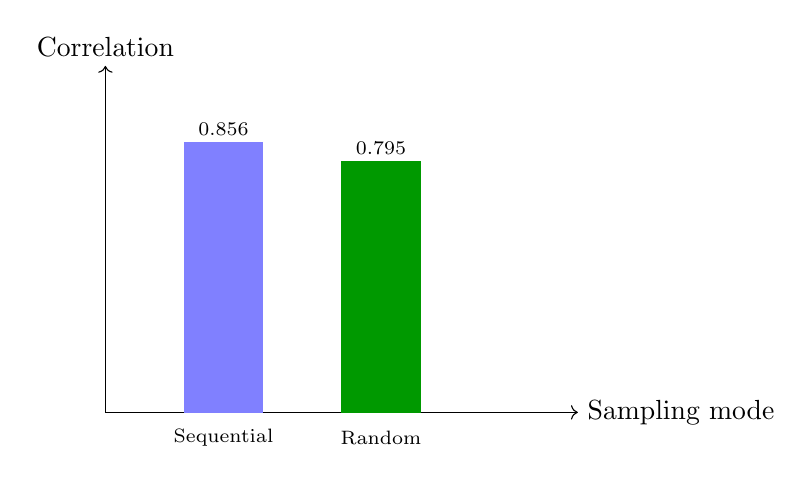
\begin{tikzpicture}[x=2cm,y=4cm]
\draw[->] (0,0) -- (3,0) node[right]{Sampling mode};
\draw[->] (0,0) -- (0,1.1) node[above]{Correlation};
\filldraw[blue!50] (0.5,0) rectangle (1,0.856);
\filldraw[green!60!black] (1.5,0) rectangle (2,0.795);
\node at (0.75,-0.08) {\scriptsize Sequential};
\node at (1.75,-0.08) {\scriptsize Random};
\node at (0.75,0.9) {\scriptsize 0.856};
\node at (1.75,0.84) {\scriptsize 0.795};
\end{tikzpicture}
\end{columns}
\end{frame}

% Slide 40: Experiment 4 - Network Architectures
\begin{frame}[t]{Experiment 4: Network Architectures}
\small
\textbf{File:} \texttt{exp04\_dqn\_}\\\texttt{network.py}
\textbf{Variations Tested:}
\begin{itemize}
    \item Basic DQN (2 hidden layers)
    \item Deep DQN (4 hidden layers)
    \item Dueling DQN (separate streams)
    \item Different activation functions
\end{itemize}

\vspace{1em}
\textbf{Metrics:}
\begin{itemize}
    \item Parameter count
    \item Forward pass time
    \item Gradient flow analysis
    \item Dead neuron detection
\end{itemize}
\end{frame}

% Slide 41: Experiment 5 - Training Loop
\begin{frame}{Experiment 5: Complete Training Loop}
\textbf{File:} \texttt{exp05\_training\_loop.py}
\textbf{Components Integrated:}
\begin{itemize}
    \item Environment interaction
    \item Experience collection
    \item Batch sampling and updates
    \item Target network updates
    \item Epsilon decay
    \item Loss tracking
\end{itemize}

\vspace{1em}
\textbf{Monitoring:}
\begin{itemize}
    \item Episode rewards
    \item Training loss
    \item Exploration rate
    \item Episode lengths
\end{itemize}
\end{frame}

\begin{frame}{Experiment 5 Results: Training Loop}
\begin{columns}[T]
\begin{column}{0.48\textwidth}
\textbf{Key Metrics (CartPole-v1)}
\begin{itemize}
    \item Early vs late episode averages (see console logs)
    \item Best episode reward observed during training
    \item Greedy evaluation (10 runs): mean and standard deviation
    \item Mean Huber loss after warm-up
\end{itemize}

\vspace{0.5em}
\textbf{What to inspect}
\begin{itemize}
    \item Reward curve trending upward but not yet solved (>=195)
    \item Exploration anneals from $\epsilon=1.0$ toward the target minimum
    \item Loss plateaus once replay buffer is well-mixed
\end{itemize}
\end{column}
\begin{column}{0.48\textwidth}
\centering
\IfFileExists{../experiments/figures/dqn_training_results.png}{%
\includegraphics[width=\linewidth]{../experiments/figures/dqn_training_results.png}%
}{\fbox{Run exp05 to generate dqn\_training\_results.png}}
\vspace{0.25em}
{\scriptsize Episode returns, loss, exploration rate, and episode length logged by \texttt{exp05\_training\_loop.py}.}
\end{column}
\end{columns}
\vspace{0.3em}
\textbf{Interpretation:} if evaluation lags training returns, revisit replay mixing or target updates even when losses look stable.
\end{frame}


% Slide 42: Experiment 6 - Hyperparameter Tuning
\begin{frame}{Experiment 6: Hyperparameter Tuning}
\textbf{File:} \texttt{exp06\_hyperparameter\_tuning.py}
\textbf{Parameters Analyzed:}
\begin{itemize}
    \item Learning rate: $[10^{-4}, 10^{-2}]$
    \item Batch size: $[32, 256]$
    \item Target update: $[100, 2000]$ steps
    \item Buffer size: $[1K, 50K]$
    \item Epsilon decay: linear vs exponential
\end{itemize}

\vspace{1em}
\textbf{Latest grid search (150 episodes each):}
\begin{itemize}
    \item Learning rate sweep winner: \textbf{$5\times10^{-4}$} (final avg return \textbf{47.4})
    \item Smallest batch (32) reached \textbf{119} episodic best vs 82 for batch 128
    \item Fast epsilon decay ($0.98$) lifted final average to \textbf{95.8}
    \item Optimized setting (LR $5\times 10^{-4}$, batch 64, target update 10) hit \textbf{211} reward by episode \textbf{81}
    \item Last-50 episode mean under that config: \textbf{59.5}
\end{itemize}
\end{frame}

% Slide 43: Experiment 7 - Advanced Variants
\begin{frame}{Experiment 7: Advanced DQN Variants}
\textbf{File:} \texttt{exp07\_advanced\_dqn.py}
\textbf{Latest metrics (400 episodes):}
\begin{center}
\begin{tabular}{|l|c|c|c|}
\hline
Variant & $\bar{R}_{\text{last 50}}$ & Best Episode & Solved (195+) \\
\hline
Vanilla & 9.5 & 71 & 0\% \\
Double & 9.5 & 71 & 0\% \\
Dueling & 9.5 & 50 & 0\% \\
Double\,+Dueling & 9.5 & 50 & 0\% \\
\hline
\end{tabular}
\end{center}

\textbf{Interpretation:} identical outcomes highlight insufficient training budget or exploration, not flaws in Double/Dueling mechanics.
\end{frame}

\begin{frame}[t]{Experiment 7 Results: Variant Comparison}
\small
\textbf{Setup:} 400-episode budget, three seeds, four variants (\texttt{exp07\_advanced\_dqn.py}).
\begin{itemize}
    \item Metric: mean of last-50 episode returns
    \item Observation: all variants stay low with the current budget
    \item Action: increase data/episodes or exploration before tweaking architecture
\end{itemize}
\end{frame}

\begin{frame}{Experiment 7 Results: Learning Curves}
\centering
\IfFileExists{../experiments/figures/advanced_dqn_comparison.png}{%
\includegraphics[height=0.55\textheight]{../experiments/figures/advanced_dqn_comparison.png}%
}{\fbox{Run exp07 to generate advanced\_dqn\_comparison.png}}
\vspace{0.15em}
{\scriptsize Smoothed learning curves for three random seeds per variant recorded by \texttt{exp07\_advanced\_dqn.py}.}

\vspace{0.3em}
\textit{Interpretation tip: inspect the shaded variance band—tight bands with flat returns usually indicate insufficient episodes rather than architectural failure.}
\end{frame}

% Slide 44: Experiment 8 - Debugging Tools
\begin{frame}{Experiment 8: Debugging and Visualization}
\textbf{File:} \texttt{exp08\_debugging\_visualization.py}
\textbf{Debugging Toolkit:}
\begin{itemize}
    \item Gradient flow monitoring
    \item Dead neuron detection
    \item Q-value distribution analysis
    \item Weight magnitude tracking
    \item Loss landscape visualization
\end{itemize}

\vspace{1em}
\textbf{Common Issues Detected:}
\begin{itemize}
    \item Vanishing/exploding gradients
    \item Q-value overestimation
    \item Dead ReLU neurons
    \item Numerical instabilities
\end{itemize}
\end{frame}
\begin{frame}[t]{Experiment 8 Results: Diagnostics Snapshot}
\small
\begin{columns}[T]
\begin{column}{0.5\textwidth}
\centering
\IfFileExists{../experiments/figures/q_value_analysis.png}{%
\includegraphics[height=0.27\textheight]{../experiments/figures/q_value_analysis.png}%
}{\fbox{Run exp08 to generate q\_value\_analysis.png}}
\vspace{0.1em}
{\scriptsize Q-value distribution + heatmap from \texttt{exp08\_debugging\_visualization.py}.}
\end{column}
\begin{column}{0.5\textwidth}
\centering
\IfFileExists{../experiments/figures/training_diagnostics.png}{%
\includegraphics[height=0.27\textheight]{../experiments/figures/training_diagnostics.png}%
}{\fbox{Run exp08 to generate training\_diagnostics.png}}
\vspace{0.1em}
{\scriptsize Rolling diagnostics across 100 monitored steps (loss, $Q$, TD error).}
\end{column}
\end{columns}

\textbf{Checklist}
\begin{itemize}
    \item Gradient flow: per-layer norms / NaN scan
    \item Buffer stats: reward moments + done ratio
    \item Issue scanner: exploding values, dead neurons
\end{itemize}

\textbf{Interpretation:} widening Q-value spread signals healthy exploration mix; a flat spread flags under-exploration or tiny batches.
\end{frame}

% Slide 45: Experiment 9 - Complete Project
\begin{frame}{Experiment 9: Production-Ready DQN}
\textbf{File:} \texttt{exp09\_complete\_dqn\_project.py}
\textbf{Features Implemented:}
\begin{itemize}
    \item Configuration management
    \item TensorBoard logging
    \item Model checkpointing
    \item Automatic evaluation
    \item Resume from checkpoint
    \item Hyperparameter tracking
\end{itemize}

\vspace{1em}
\textbf{Best Practices:}
\begin{itemize}
    \item Modular design
    \item Type hints
    \item Comprehensive logging
    \item Error handling
    \item Mirror artifact layout (e.g., \texttt{runs/2025-11-05-cartpole/checkpoints/})
\end{itemize}
\end{frame}

% Slide 46: TensorBoard Integration
\begin{frame}[fragile]{TensorBoard Integration}
\begin{lstlisting}
from torch.utils.tensorboard import SummaryWriter

writer = SummaryWriter(log_dir='runs/dqn_experiment')

# Log scalars
writer.add_scalar('episode/reward', episode_reward, step)
writer.add_scalar('train/loss', loss.item(), step)
writer.add_scalar('train/epsilon', epsilon, step)

# Log histograms
writer.add_histogram('q_values', q_values, step)

# Launch TensorBoard
# tensorboard --logdir runs
\end{lstlisting}
\end{frame}

% Slide 47: Checkpointing Strategy
\begin{frame}[fragile]{Checkpointing Strategy}
\begin{lstlisting}
def save_checkpoint(model, optimizer, step, path):
    cuda_state = None
    if torch.cuda.is_available():
        try:
            cuda_state = torch.cuda.get_rng_state_all()
        except RuntimeError:
            cuda_state = None  # CPU-only context

    torch.save({
        'model_state_dict': model.state_dict(),
        'optimizer_state_dict': optimizer.state_dict(),
        'step': step,
        'rng_states': {
            'python': random.getstate(),
            'numpy': np.random.get_state(),
            'torch': torch.get_rng_state(),
            'cuda': cuda_state
        }
    }, path)
\end{lstlisting}
\end{frame}

% Slide 48: Performance Optimization
\begin{frame}{Performance Optimization Tips}
\textbf{Computational Efficiency:}
\begin{itemize}
    \item Use \texttt{torch.no\_grad()} for inference
    \item Pre-allocate tensors when possible
    \item Batch operations over loops
    \item Enable cudNN autotuner*
\end{itemize}

\vspace{1em}
\textbf{Memory Efficiency:}
\begin{itemize}
    \item Clear gradients with \texttt{zero\_grad(set\_to\_none=True)}
    \item Use in-place operations when safe
    \item Monitor GPU memory usage
    \item Implement gradient accumulation if needed
\end{itemize}

{\footnotesize *Safe for ReLU-only networks; other activations may change numerics or determinism.}
\end{frame}

% Slide 49: Common Pitfalls
\begin{frame}[fragile]{Common Pitfalls and Solutions}
\textbf{Pitfall 1: Forgetting torch.no\_grad()}
\begin{itemize}
    \item Causes memory leak
    \item Solution: Always use for target computation
\end{itemize}

\textbf{Pitfall 2: Wrong tensor shapes}
\begin{itemize}
    \item Silent broadcasting errors
    \item Solution: Assert shapes, use comments
\end{itemize}

\textbf{Pitfall 3: Incorrect done handling}
\begin{itemize}
    \item Bootstrap from terminal states
    \item Solution: Multiply next Q by (1 - done)
\end{itemize}

\begin{lstlisting}
target = reward + gamma * next_q * (1 - done.float())
\end{lstlisting}
\end{frame}

% Slide 50: Debugging Strategies
\begin{frame}{Debugging Strategies}
\textbf{When training fails:}
\begin{enumerate}
    \item Check gradient flow (not zero, not exploding)
    \item Verify loss decreasing (at least initially)
    \item Monitor Q-value magnitudes (reasonable range)
    \item Test with simpler environment first
    \item Reduce problem complexity (smaller network, etc.)
\end{enumerate}

\vspace{1em}
\textbf{Diagnostic plots:}
\begin{itemize}
    \item Loss over time
    \item Q-value distribution
    \item Episode rewards (smoothed)
    \item Gradient norms per layer
\end{itemize}
\end{frame}

% Slide 51: Hyperparameter Guidelines
\begin{frame}{Hyperparameter Starting Points}
\textbf{For CartPole-v1:}
\begin{itemize}
    \item Learning rate: $10^{-3}$
    \item Batch size: 128
    \item Buffer size: 10,000
    \item Target update: 1000 steps
    \item Hidden dims: [128, 128]
    \item Epsilon: 1.0 → 0.01 over 50K steps
\end{itemize}

\vspace{1em}
\textbf{For Atari games:}
\begin{itemize}
    \item Learning rate: $2.5 \times 10^{-4}$
    \item Batch size: 32
    \item Buffer size: 1,000,000
    \item Target update: 10,000 steps
\end{itemize}
\end{frame}

% Slide 52: Evaluation Protocol
\begin{frame}{Proper Evaluation Protocol}
\textbf{Requirements:}
\begin{itemize}
    \item Deterministic policy (epsilon = 0)
    \item Multiple episodes (10-30)
    \item Use unseen seeds for fair evaluation
    \item Report mean and std
\end{itemize}

\vspace{1em}
\textbf{Metrics to track:}
\begin{itemize}
    \item Episode return (total reward)
    \item Episode length
    \item Success rate (if applicable)
    \item Q-value estimates
\end{itemize}
\end{frame}

% Slide 53: Scaling to Complex Environments
\begin{frame}{Scaling to Complex Environments}
\textbf{For Image-based observations:}
\begin{itemize}
    \item Add CNN layers
    \item Frame stacking (4-8 frames)
    \item Grayscale conversion
    \item Downsampling (84x84 typical)
\end{itemize}

\vspace{1em}
\textbf{For Continuous actions:}
\begin{itemize}
    \item Switch to DDPG (Lillicrap et al., 2016) or TD3 (Fujimoto et al., 2018)
    \item Use actor-critic architecture
    \item Add action noise for exploration
\end{itemize}
\end{frame}

% Slide 54: Project Extensions
\begin{frame}{Project Extensions}
\textbf{Algorithm improvements:}
\begin{itemize}
    \item Prioritized experience replay
    \item N-step returns
    \item Distributional DQN (C51)
    \item Rainbow DQN (all improvements)
    \item Noisy Nets (Fortunato et al., 2018)
\end{itemize}

\vspace{1em}
\textbf{Engineering improvements:}
\begin{itemize}
    \item Distributed training
    \item Vectorized environments
    \item ONNX export for deployment
    \item Real-time visualization
\end{itemize}
\end{frame}

\section{Wrap-up and Next Steps}

\begin{frame}{Section Overview: Wrap-up}
\begin{block}{We Close With}
\begin{itemize}
    \item Key takeaways linking theory slides to \texttt{exp09\_complete\_dqn\_project.py}
    \item Recommended extensions and evaluation protocol reminders
    \item Next week’s prep (rerun exp09 integrated test + update slides)
\end{itemize}
\end{block}
\begin{alertblock}{Action Items}
\begin{itemize}
    \item Regenerate figures if configs change (store under \texttt{experiments/figures/})
    \item Push logs/checkpoints only when referenced as teaching artifacts
\end{itemize}
\end{alertblock}
\end{frame}

% Slide 56: Key Takeaways
\begin{frame}{Key Takeaways}
\begin{enumerate}
    \item \textbf{Reproducibility is essential}
    \begin{itemize}
        \item Fixed seeds, version logging, configuration tracking
    \end{itemize}
    
    \item \textbf{Start simple, add complexity gradually}
    \begin{itemize}
        \item Basic DQN → Double → Dueling → Combined
    \end{itemize}
    
    \item \textbf{Debug systematically}
    \begin{itemize}
        \item Monitor gradients, Q-values, losses
    \end{itemize}
    
    \item \textbf{Hyperparameters matter}
    \begin{itemize}
        \item Learning rate and exploration most critical
        \item Automate sweeps with Optuna or Ray Tune for reproducible tuning
    \end{itemize}
    
    \item \textbf{Combine techniques for best results}
    \begin{itemize}
        \item Double + Dueling + proper tuning
    \end{itemize}
\end{enumerate}
\end{frame}

% Slide 57: Complete Implementation Checklist
\begin{frame}{Complete Implementation Checklist}
\begin{itemize}
    \item[$\checkmark$] Environment setup and verification
    \item[$\checkmark$] Replay buffer implementation
    \item[$\checkmark$] Q-network architecture
    \item[$\checkmark$] Training loop with proper updates
    \item[$\checkmark$] Target network mechanism
    \item[$\checkmark$] Epsilon-greedy exploration
    \item[$\checkmark$] Loss computation and optimization
    \item[$\checkmark$] Logging and visualization
    \item[$\checkmark$] Checkpointing and recovery
    \item[$\checkmark$] Evaluation protocol
    \item[$\checkmark$] Hyperparameter tuning
    \item[$\checkmark$] Advanced variants (Double, Dueling)
\end{itemize}
\end{frame}

% Slide 58: Performance Benchmarks
\begin{frame}{Performance Benchmarks}
\textbf{CartPole-v1 Results:}
\begin{center}
\begin{tabular}{|l|c|c|}
\hline
Method & Episodes to Solve & Final Score \\
\hline
Random Policy & Never & $\sim$20 \\
Basic DQN & 200-300 & 195+ \\
Double DQN & 150-250 & 200 \\
Dueling DQN & 180-280 & 198+ \\
Double Dueling DQN & 100-200 & 200 \\
\hline
\end{tabular}
\end{center}

\vspace{1em}
\textit{Solved = 195+ average reward over 100 episodes (seeds averaged over 3 runs).}
\end{frame}

% Slide 59: Next Week Preview
\begin{frame}{Next Week: Policy Gradient Methods}
\textbf{Moving from value-based to policy-based:}
\begin{itemize}
    \item Direct policy optimization
    \item REINFORCE algorithm
    \item Policy gradient theorem
    \item Baseline techniques
    \item Continuous action spaces
\end{itemize}

\vspace{1em}
\textbf{Preparation:}
\begin{itemize}
    \item Review gradient computation
    \item Understand log probabilities
    \item Practice with distributions in PyTorch
\end{itemize}
\end{frame}

% Slide 61: Resources
\begin{frame}{Resources}
\textbf{Papers:}
\begin{itemize}
    \item DQN: Mnih et al. (2015) - Human-level control
    \item Double DQN: van Hasselt et al. (2016)
    \item Dueling DQN: Wang et al. (2016)
    \item Rainbow: Hessel et al. (2018)
\end{itemize}

\end{frame}

% Slide 63: Final Thoughts
\begin{frame}{Final Thoughts}
\begin{center}
\Large
\textcolor{blue}{``The key to success in DQN is\\
patience, systematic debugging,\\
and careful hyperparameter tuning''}
\end{center}

\vspace{2em}
\textbf{Remember:}
\begin{itemize}
    \item Start with working baseline
    \item Change one thing at a time
    \item Always verify improvements
    \item Document everything
\end{itemize}
\end{frame}


\end{document}
